\chapter{Time Systems in Celestial Mechanics}
\label{ch:time_systems}

Time measurement is fundamental to celestial mechanics, yet surprisingly complex. Different applications require different time scales, each with specific definitions and use cases. This chapter describes the time systems implemented in AstDyn and their interconversions.

\section{Why Multiple Time Systems?}

A naive approach might use ordinary civil time (UTC) for all calculations. However, this is inadequate for precision celestial mechanics due to:

\begin{itemize}
    \item \textbf{Earth's irregular rotation}: The length of a day varies due to tidal friction, atmospheric effects, and core-mantle coupling
    \item \textbf{Leap seconds}: UTC includes discontinuous jumps to stay synchronized with Earth's rotation
    \item \textbf{Relativistic effects}: Time flows differently in different gravitational potentials
    \item \textbf{Precision requirements}: Sub-second accuracy over centuries demands careful timekeeping
\end{itemize}

\section{Julian Day Number}

Before discussing specific time scales, we introduce the Julian Day (JD) system, a continuous count of days since noon UTC on January 1, 4713 BCE (proleptic Julian calendar).

\begin{definition}[Julian Day]
The Julian Day Number (JD) is the number of days elapsed since the epoch JD 0.0 = 12:00 UT on January 1, 4713 BCE.
\end{definition}

For example:
\begin{itemize}
    \item January 1, 2000, 12:00 TT = JD 2451545.0
    \item November 26, 2025, 00:00 UTC $\approx$ JD 2460638.5
\end{itemize}

\subsection{Modified Julian Day}

To reduce numerical precision requirements, the \textit{Modified Julian Day} (MJD) is commonly used:

\begin{equation}
\text{MJD} = \text{JD} - 2400000.5
\end{equation}

This shifts the epoch to November 17, 1858, 00:00 UTC, and starts days at midnight rather than noon. The reference epoch J2000.0 corresponds to:

\begin{equation}
\text{MJD}_{\text{J2000}} = 51544.5
\end{equation}

AstDyn primarily uses MJD for internal calculations.

\section{Universal Time (UT)}

Universal Time (UT) is based on Earth's rotation. Several variants exist:

\subsection{UT0}

UT0 is raw Universal Time as measured by observing stellar positions. It varies due to polar motion (wobble of Earth's rotation axis).

\subsection{UT1}

UT1 corrects UT0 for polar motion effects:

\begin{equation}
\text{UT1} = \text{UT0} + \Delta \lambda
\end{equation}

where $\Delta\lambda$ accounts for the shift in observer's longitude due to polar motion. UT1 represents the true rotational angle of the Earth.

\subsection{UTC (Coordinated Universal Time)}

UTC is the civil time standard, defined by atomic clocks but kept within 0.9 seconds of UT1 by inserting \textit{leap seconds}. The difference is:

\begin{equation}
\Delta UT = \text{UT1} - \text{UTC}
\end{equation}

Leap seconds are announced by the International Earth Rotation Service (IERS) and typically occur on June 30 or December 31.

\begin{figure}[H]
\centering
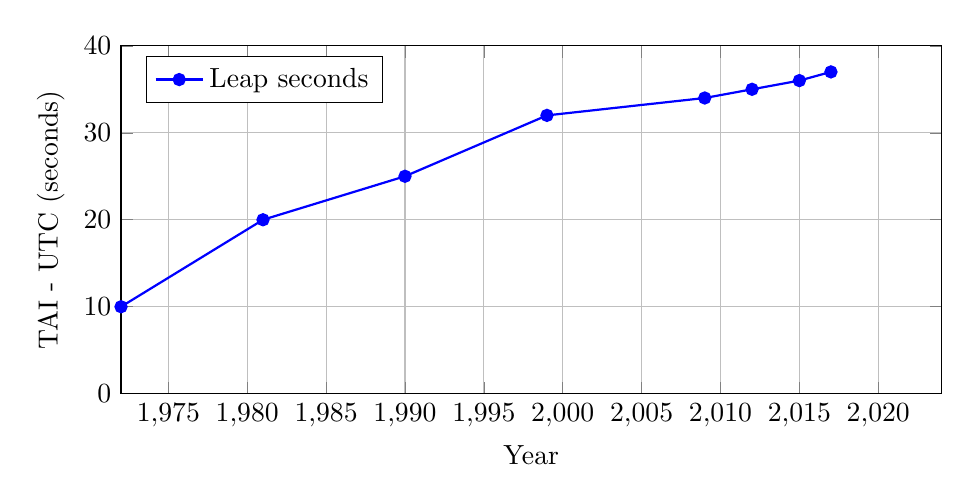
\begin{tikzpicture}
    \begin{axis}[
        width=12cm,
        height=6cm,
        xlabel={Year},
        ylabel={TAI - UTC (seconds)},
        xmin=1972,
        xmax=2024,
        ymin=0,
        ymax=40,
        grid=major,
        legend pos=north west
    ]
    \addplot[blue, thick, mark=*] coordinates {
        (1972,10) (1981,20) (1990,25) (1999,32)
        (2009,34) (2012,35) (2015,36) (2017,37)
    };
    \legend{Leap seconds}
    \end{axis}
\end{tikzpicture}
\caption{Accumulation of leap seconds since 1972}
\label{fig:leapseconds}
\end{figure}

\section{Atomic Time Scales}

\subsection{TAI (International Atomic Time)}

TAI is a continuous, uniform time scale defined by an ensemble of atomic clocks worldwide. It has no leap seconds and forms the basis for other modern time scales.

The relationship to UTC is:

\begin{equation}
\text{TAI} = \text{UTC} + \Delta AT
\end{equation}

where $\Delta AT$ is the cumulative number of leap seconds (37 seconds as of 2024).

\subsection{TT (Terrestrial Time)}

Terrestrial Time is the theoretical time scale for observations at Earth's surface. It is related to TAI by a constant offset:

\begin{equation}
\text{TT} = \text{TAI} + 32.184 \text{ s}
\end{equation}

The 32.184-second offset was chosen to maintain continuity with the old Ephemeris Time (ET) scale. TT is the time argument for geocentric ephemerides.

\subsection{TDB (Barycentric Dynamical Time)}

Barycentric Dynamical Time is the time scale for calculations at the solar system barycenter (center of mass). Due to general relativistic effects, time flows at different rates in different gravitational potentials.

The relationship between TDB and TT includes both periodic and secular terms:

\begin{equation}
\text{TDB} = \text{TT} + 0.001658 \sin(g) + 0.000014 \sin(2g) \text{ seconds}
\end{equation}

where $g$ is the mean anomaly of Earth's orbit around the Sun:

\begin{equation}
g = 357.53° + 0.9856003°(JD - 2451545.0)
\end{equation}

This correction is typically a few milliseconds but accumulates over long time spans.

\section{Time Scale Relationships}

Figure~\ref{fig:timescales} illustrates the relationships between time scales:

\begin{figure}[H]
\centering
\resizebox{\columnwidth}{!}{%
\begin{tikzpicture}[
    node distance=2.5cm,
    box/.style={rectangle, draw, fill=blue!10, text width=2cm, align=center, minimum height=1cm},
    arrow/.style={->, >=stealth, thick}
]
    \node[box] (utc) {UTC};
    \node[box, right=of utc] (tai) {TAI};
    \node[box, right=of tai] (tt) {TT};
    \node[box, right=of tt] (tdb) {TDB};
    \node[box, below=of utc] (ut1) {UT1};
    
    \draw[arrow] (utc) -- node[above] {\small $+\Delta AT$} (tai);
    \draw[arrow] (tai) -- node[above] {\small $+32.184$ s} (tt);
    \draw[arrow] (tt) -- node[above] {\small $+\Delta T_{rel}$} (tdb);
    \draw[arrow] (utc) -- node[left] {\small $+\Delta UT$} (ut1);
\end{tikzpicture}%
}
\caption{Relationships between major time scales}
\label{fig:timescales}
\end{figure}

\section{Implementation in AstDyn}

The \texttt{TimeScale} class handles conversions between time systems:

\begin{lstlisting}[style=cpp,caption={Time scale conversions}]
#include <astdyn/time/TimeScale.hpp>
using namespace astdyn::time;

// UTC to TDB conversion
double mjd_utc = 61000.0;
double mjd_tdb = TimeScale::utc_to_tdb(mjd_utc);

// TT to TAI
double mjd_tt = 61000.0;
double mjd_tai = TimeScale::tt_to_tai(mjd_tt);

// UT1 to UTC (requires Delta_UT from IERS)
double delta_ut = 0.15;  // seconds, from IERS Bulletin A
double mjd_ut1 = 61000.0;
double mjd_utc_computed = mjd_ut1 - delta_ut / 86400.0;
\end{lstlisting}

\subsection{Leap Second Table}

AstDyn maintains an internal table of leap seconds, updated periodically:

\begin{table}[H]
\centering
\caption{Recent leap seconds (partial table)}
\label{tab:leapseconds}
\begin{tabular}{@{}lcc@{}}
\toprule
\textbf{Date} & \textbf{MJD} & \textbf{TAI-UTC (s)} \\
\midrule
2012-07-01 & 56109 & 35 \\
2015-07-01 & 57204 & 36 \\
2017-01-01 & 57754 & 37 \\
\bottomrule
\end{tabular}
\end{table}

\subsection{$\Delta T$ Approximations}

For historical dates or future predictions where leap seconds are unknown, empirical formulas approximate $\Delta T = \text{TT} - \text{UT}$:

\textbf{Before 1972} (polynomial fit):
\begin{equation}
\Delta T \approx -20 + 32t^2 \text{ seconds}
\end{equation}
where $t$ is centuries from 1820.

\textbf{After 2015} (linear extrapolation):
\begin{equation}
\Delta T \approx 69.2 + 0.4 \times (y - 2015) \text{ seconds}
\end{equation}
where $y$ is the year.

These approximations have uncertainties of several seconds and should not be used for precise work.

\section{Practical Considerations}

\subsection{Which Time Scale to Use?}

\begin{description}
    \item[Observations] Use UTC for recording observation times (easily synchronized with GPS)
    \item[Orbit calculations] Convert to TDB for numerical integration
    \item[Earth rotation] Use UT1 for computing sidereal time and topocentric coordinates
    \item[Reporting] Use UTC for disseminating results to observers
\end{description}

\subsection{Precision Requirements}

For typical asteroid orbit determination:
\begin{itemize}
    \item Position accuracy: $\sim 0.1''$ (arcsecond)
    \item Time accuracy needed: $\sim 0.01$ s
    \item Effect of 1-second time error: $\sim 15''$ in RA for main-belt asteroid
\end{itemize}

Therefore, using the correct time scale and accounting for leap seconds is essential.

\subsection{Example: Time Conversion Chain}

Complete conversion from civil date to TDB:

\begin{lstlisting}[style=cpp,caption={Converting calendar date to TDB}]
// Input: UTC civil date
int year = 2025, month = 11, day = 26;
double hour = 12.5;  // 12:30 UT

// Step 1: Calendar to Julian Day
double jd_utc = calendar_to_jd(year, month, day + hour/24.0);
double mjd_utc = jd_utc - 2400000.5;

// Step 2: UTC to TDB
double mjd_tdb = TimeScale::utc_to_tdb(mjd_utc);

std::cout << "MJD (TDB): " << std::fixed << std::setprecision(6) 
          << mjd_tdb << std::endl;
// Output: MJD (TDB): 61000.520833
\end{lstlisting}

\section{Further Reading}

Detailed specifications of time systems are maintained by:
\begin{itemize}
    \item \textbf{IERS} (International Earth Rotation Service): \url{https://www.iers.org}
    \item \textbf{BIPM} (International Bureau of Weights and Measures): TAI definition
    \item \textbf{IAU} (International Astronomical Union): Resolutions on time scales
    \item \textbf{USNO} (US Naval Observatory): \textit{Astronomical Almanac}
\end{itemize}

The SOFA library (Standards of Fundamental Astronomy) provides reference implementations of time and coordinate transformations: \url{http://www.iausofa.org}
